\documentclass[12pt,hyperref,a4paper,UTF8,twoside]{ctexart}
\usepackage{XTUReport}
\usepackage{tikz}
\usetikzlibrary{arrows.meta,calc}

\newcommand{\curl}{\operatorname{curl}}
\newcommand{\diverge}{\operatorname{div}}
\newcommand{\E}{\bm{E}}
\newcommand{\Hfield}{\bm{H}}
\newcommand{\J}{\bm{J}}
\newcommand{\n}{\bm{n}}
\newcommand{\tvec}{\bm{t}}
\newcommand{\R}{\mathbb{R}}

\setlength{\headheight}{15pt}
\begin{document}
\cover%封面
\thispagestyle{empty}
%中文摘要
\newpage
\pagestyle{abstractcnstyle}
\pagenumbering{Roman}
\begin{abstractcn}

本文以二维频域 Maxwell 方程为研究对象,围绕 $H(\text{curl})$ 空间、弱形式推导、Nédélec 边缘元离散以及稀疏矩阵实现展开讨论.通过将完整三维电磁问题简化为二维有界区域上的双旋方程,本文保留了 Maxwell 方程的核心旋度结构,同时降低了函数空间与有限元构造的复杂度.文中首先建立带理想电导体边界条件的二维强形式模型,随后在 $H_0(\text{curl};\Omega)$ 空间中推导相应弱形式,并说明 Nédélec 边缘元相较于传统节点元在保持切向连续性和避免伪模态方面的优势.最后,结合三角剖分、边自由度、稀疏矩阵组装、数值实验和先验误差分析,给出二维计算电磁问题的一套较完整的理论与实现框架.数值结果表明,最低阶 Nédélec 边缘元在光滑制造解算例中呈现接近一阶的收敛行为.

\end{abstractcn}
\keywordscn{二维 Maxwell 方程；$H(\text{curl})$ 空间；Nédélec 边缘元；有限元方法；稀疏矩阵}

%英文摘要
\newpage
\pagestyle{abstractenstyle}
\begin{abstracten}
This report studies a two-dimensional frequency-domain Maxwell problem and its finite element discretization in the $H(\text{curl})$ framework. By reducing the full three-dimensional electromagnetic model to a two-dimensional double-curl equation, the essential curl structure is preserved while the mathematical and computational complexity is reduced. The strong form with perfect electric conductor boundary conditions is first introduced, followed by the weak formulation in $H_0(\text{curl};\Omega)$. The lowest-order Nédélec edge element on triangular meshes is then used to construct a conforming discretization. Sparse matrix assembly, numerical convergence tests, linear solver choices, and a priori error estimates are also discussed. The resulting framework provides a clear entry point for understanding edge-element methods in computational electromagnetics.
\end{abstracten}
\keywordsen{two-dimensional Maxwell equations; $H(\text{curl})$ space; Nédélec edge element; finite element method; sparse matrix}

\newpage
\pagestyle{contentstyle}
\tableofcontents

\newpage
\pagestyle{articlestyle} % 切换回正文页眉样式
\pagenumbering{arabic} % 设置页码样式为阿拉伯数字
\setcounter{page}{1}   % 正文页码从1开始



\section{引言}

在计算电磁学中,高频谐振腔、波导结构以及散射问题中的电磁场分布通常由频域 Maxwell 方程描述.与低频静态问题不同,高频问题中电场与磁场相互耦合,波动效应、边界反射以及介质界面处的传播特性都会显著影响数值解的精度.因此,如何构造既符合电磁场物理规律,又具有良好数值稳定性的离散格式,是有限元方法应用于 Maxwell 方程时的核心问题之一.

完整的 Maxwell 方程本质上是三维向量场问题,其函数空间、边界迹和有限元构造都较为复杂.为了降低分析和实现难度,同时保留问题中最重要的旋度结构,本文选取二维频域 Maxwell 模型作为研究对象.设计算区域为有界 Lipschitz 区域
\[
\Omega\subset\R^2,
\]
电场写成平面向量场
\[
\E=(E_1,E_2)^T.
\]
二维模型虽然是对三维电磁问题的简化,但仍然包含 $H(\text{curl})$ 空间、切向连续性、理想电导体边界条件以及 Nédélec 边缘元等关键内容,因此非常适合作为学习 Maxwell 有限元离散的基础模型.

在电磁问题中,电场在介质界面上的连续性与标量椭圆方程有本质区别.特别地,电场的切向分量需要满足适当的连续条件,而法向分量在介质参数不连续时可以发生跳跃.这意味着电场并不天然属于传统的 $[H^1(\Omega)]^2$ 协调空间.若强行采用节点有限元来逼近电场,就会人为施加过强的连续性要求,从而破坏真实电磁场的界面性质,并可能在本征值问题中产生非物理伪模态.

因此,Maxwell 方程的自然函数空间不是 $H^1$ 空间,而是与旋度算子相适应的 $H(\text{curl};\Omega)$ 空间.该空间只要求向量场本身及其旋度平方可积,不要求所有一阶偏导数都平方可积,因而更符合电磁场的物理正则性.相应地,有限元离散也应采用 $H(\text{curl})$ 协调的 Nédélec 边缘元.与节点元以节点函数值作为自由度不同,Nédélec 元以边上的切向积分作为自由度,能够自然保持跨单元边界的切向连续性,同时允许法向分量不连续.

本文围绕二维频域 Maxwell 方程展开.首先,建立带理想电导体(PEC)边界条件的二维强形式模型；其次,在 $H_0(\text{curl};\Omega)$ 空间中推导弱形式；然后,采用三角剖分上的最低阶第一类 Nédélec 边缘元进行离散；最后,从稀疏矩阵组装、线性系统求解和先验误差分析等角度讨论其数值实现与理论性质.通过该二维模型,可以较清晰地理解 Nédélec 边缘元在计算电磁学中的数学基础和工程实现方法.

\section{强形式与数学模型}

考虑一个由理想导体包裹的二维有界 Lipschitz 区域
\[
\Omega\subset\R^2,
\qquad
\Gamma=\partial\Omega.
\]
该区域可以看作二维截面上的谐振腔或波导简化模型.假设场量具有时谐因子 $e^{j\omega t}$,其中 $\omega$ 为角频率,$j=\sqrt{-1}$.在频域下,时间微分可转化为乘以 $j\omega$,从而得到仅依赖空间变量的复值方程.

在二维情形中,平面向量场的旋度定义为标量:
\[
\curl \E
=
\frac{\partial E_2}{\partial x}
-
\frac{\partial E_1}{\partial y}.
\]
另一方面,对于标量函数 $\phi$,定义其旋度为二维向量:
\[
\curl \phi
=
\begin{pmatrix}
\dfrac{\partial \phi}{\partial y}\\[4pt]
-\dfrac{\partial \phi}{\partial x}
\end{pmatrix}.
\]
因此,$\curl\E$ 是标量,而 $\curl(\mu_r^{-1}\curl\E)$ 又是二维向量.这种记号使二维双旋方程仍可写成与三维形式相近的表达.

令
\[
k_0=\omega\sqrt{\mu_0\varepsilon_0},
\qquad
Z_0=\sqrt{\frac{\mu_0}{\varepsilon_0}},
\]
其中 $k_0$ 为真空波数,$Z_0$ 为真空波阻抗.设 $\mu_r$ 和 $\varepsilon_r$ 分别为相对磁导率和相对介电常数.为简化讨论,本文主要考虑各向同性介质,即 $\mu_r,\varepsilon_r$ 为标量函数,并假设
\[
\mu_r,\varepsilon_r\in L^\infty(\Omega),
\qquad
\mu_r(\bm{x})\ge \alpha_\mu>0,\quad
\varepsilon_r(\bm{x})\ge \alpha_\varepsilon>0
\]
几乎处处成立.该条件保证材料参数有界且不退化.

二维频域 Maxwell 双旋方程的强形式写为
\begin{equation}
\label{eq:strong_form}
\begin{cases}
\curl\left(\mu_r^{-1}\curl \E\right)
-
k_0^2\varepsilon_r \E
=
-jk_0Z_0\J,
& \text{在 } \Omega \text{ 中},\\[4pt]
\tvec\cdot\E=0,
& \text{在 } \Gamma \text{ 上}.
\end{cases}
\end{equation}
其中 $\J=(J_1,J_2)^T$ 为外加电流密度,$\tvec$ 为边界 $\Gamma$ 上的单位切向量.边界条件
\[
\tvec\cdot\E=0
\]
表示理想电导体(Perfect Electric Conductor, PEC)边界条件,即电场沿导体表面的切向分量为零.在二维情形中,这一条件是三维 PEC 条件 $\n\times\E=\mathbf{0}$ 的平面化表达.

方程 \eqref{eq:strong_form} 中,第一项
\[
\curl(\mu_r^{-1}\curl \E)
\]
反映了磁响应和旋度传播效应；第二项
\[
k_0^2\varepsilon_r\E
\]
反映介质极化和波数对电场分布的影响；右端项
\[
-jk_0Z_0\J
\]
表示外加电流源对电磁场的激励.当 $\J=\mathbf{0}$ 时,该模型可用于讨论封闭腔体的本征振荡；当 $\J\ne\mathbf{0}$ 时,则对应受迫频域响应问题.

需要指出的是,强形式要求 $\E$ 具有足够高的经典可微性,使得双旋算子能够逐点定义.然而,在非光滑区域、凹角区域或材料参数分片不连续的情况下,电场往往不具备这样的正则性.因此,强形式主要用于描述物理模型,而数值离散前应将其转化为定义在 $H(\text{curl};\Omega)$ 空间上的弱形式.

\section{弱形式与空间分析}

为了建立严谨的变分形式,不能只在普通的平方可积空间中讨论电场.若仅要求 $\E\in [L^2(\Omega)]^2$,则 $\curl\E$ 未必有平方可积意义；若要求 $\E\in [H^1(\Omega)]^2$,又会对电场施加过强的连续性条件.二维 Maxwell 方程的自然能量空间是 $H(\text{curl};\Omega)$.

\begin{Definition}[二维 Sobolev 旋度空间]
定义
\[
H(\text{curl};\Omega)
=
\left\{
\bm{v}\in [L^2(\Omega)]^2
\mid
\curl\bm{v}\in L^2(\Omega)
\right\}.
\]
其范数为
\[
\|\bm{v}\|_{H(\text{curl};\Omega)}
=
\left(
\|\bm{v}\|_{[L^2(\Omega)]^2}^2
+
\|\curl\bm{v}\|_{L^2(\Omega)}^2
\right)^{1/2},
\]
内积为
\[
(\bm{u},\bm{v})_{H(\text{curl})}
=
\int_\Omega
\bm{u}\cdot\overline{\bm{v}}\,d\Omega
+
\int_\Omega
(\curl\bm{u})\,\overline{\curl\bm{v}}\,d\Omega.
\]
满足零切向边界条件的子空间定义为
\[
H_0(\text{curl};\Omega)
=
\left\{
\bm{v}\in H(\text{curl};\Omega)
\mid
\tvec\cdot\bm{v}=0 \text{ on } \Gamma
\right\}.
\]
这里的边界条件应理解为切向迹意义下的边界条件,而不是必须逐点成立的经典条件.
\end{Definition}

令
\[
V=H_0(\text{curl};\Omega).
\]
对强形式 \eqref{eq:strong_form} 乘以测试函数 $\bm{v}\in V$ 的共轭并在 $\Omega$ 上积分,得到
\[
\int_\Omega
\curl(\mu_r^{-1}\curl\E)\cdot\overline{\bm{v}}\,d\Omega
-
k_0^2
\int_\Omega
\varepsilon_r\E\cdot\overline{\bm{v}}\,d\Omega
=
\int_\Omega
-jk_0Z_0\J\cdot\overline{\bm{v}}\,d\Omega.
\]
二维旋度 Green 公式给出
\[
\int_\Omega
\curl\phi\cdot\overline{\bm{v}}\,d\Omega
=
\int_\Omega
\phi\,\overline{\curl\bm{v}}\,d\Omega
+
\int_\Gamma
\phi\,\overline{\bm{v}\cdot\tvec}\,dS.
\]
令 $\phi=\mu_r^{-1}\curl\E$,并利用 $\bm{v}\in H_0(\text{curl};\Omega)$,即 $\bm{v}\cdot\tvec=0$,边界项消失.因此得到弱形式:
\begin{equation}
\label{eq:weak_form}
a(\E,\bm{v})=f(\bm{v}),
\qquad \forall \bm{v}\in V,
\end{equation}
其中
\[
a(\E,\bm{v})
=
\int_\Omega
\mu_r^{-1}
(\curl\E)\,\overline{\curl\bm{v}}\,d\Omega
-
k_0^2
\int_\Omega
\varepsilon_r
\E\cdot\overline{\bm{v}}\,d\Omega,
\]
\[
f(\bm{v})
=
\int_\Omega
-jk_0Z_0
\J\cdot\overline{\bm{v}}\,d\Omega.
\]

\begin{Theorem}[弱形式的连续性]
若 $\mu_r^{-1},\varepsilon_r\in L^\infty(\Omega)$ 且 $\J\in [L^2(\Omega)]^2$,则 $a(\cdot,\cdot)$ 是 $V$ 上连续的 sesquilinear form,$f$ 是 $V$ 上连续的线性泛函.
\end{Theorem}

\begin{proof}
由 Cauchy--Schwarz 不等式及 $\mu_r^{-1},\varepsilon_r$ 的有界性可得
\[
|a(\bm{u},\bm{v})|
\le
C_\mu
\|\curl\bm{u}\|_{L^2(\Omega)}
\|\curl\bm{v}\|_{L^2(\Omega)}
+
k_0^2C_\varepsilon
\|\bm{u}\|_{[L^2(\Omega)]^2}
\|\bm{v}\|_{[L^2(\Omega)]^2}.
\]
因此存在常数 $C>0$,使得
\[
|a(\bm{u},\bm{v})|
\le
C
\|\bm{u}\|_{H(\text{curl};\Omega)}
\|\bm{v}\|_{H(\text{curl};\Omega)}.
\]
同理,
\[
|f(\bm{v})|
\le
k_0Z_0
\|\J\|_{[L^2(\Omega)]^2}
\|\bm{v}\|_{[L^2(\Omega)]^2}
\le
C
\|\bm{v}\|_{H(\text{curl};\Omega)}.
\]
故 $a$ 与 $f$ 均连续.
\end{proof}

需要注意的是,由于双线性型中含有负的零阶项
\[
-k_0^2\int_\Omega\varepsilon_r|\E|^2\,d\Omega,
\]
问题一般不满足标准 Lax--Milgram 引理中的强制性条件.因此,频域 Maxwell 问题通常应从 Fredholm 理论角度分析.若工作波数 $k_0$ 不对应腔体的谐振频率,则齐次问题只有零解,非齐次问题存在唯一解；若 $k_0$ 恰好落在谱点上,则解可能不唯一,或需要额外相容性条件.

\section{有限元离散化:Nédélec 边缘元}

弱形式 \eqref{eq:weak_form} 的解空间为 $H_0(\text{curl};\Omega)$,因此离散空间也必须保持 $H(\text{curl})$ 协调性.本文采用二维三角剖分上的最低阶第一类 Nédélec 边缘元.设
\[
\mathcal{T}_h=\{K\}
\]
为区域 $\Omega$ 的三角剖分,$h$ 为最大单元直径.每个三角形 $K$ 有三条边,因此最低阶边缘元在每个单元上有三个局部自由度.

为了说明边自由度的几何意义,图 \ref{fig:edge_mesh} 给出一个二维三角剖分示意图.箭头表示每条边的局部方向,边上的切向积分即为 Nédélec 元的自由度.

\begin{figure}[htbp]
\centering
\begin{tikzpicture}[scale=1.1, >=Stealth]
\coordinate (A) at (0,0);
\coordinate (B) at (2,0);
\coordinate (C) at (4,0);
\coordinate (D) at (0.8,1.5);
\coordinate (E) at (2.8,1.6);
\coordinate (F) at (1.8,3.0);

\draw[thick] (A)--(B)--(D)--cycle;
\draw[thick] (B)--(E)--(D)--cycle;
\draw[thick] (B)--(C)--(E)--cycle;
\draw[thick] (D)--(E)--(F)--cycle;
\draw[very thick] (A)--(B)--(C)--(E)--(F)--(D)--cycle;

\draw[->, thick] ($(A)!0.25!(B)$) -- ($(A)!0.75!(B)$);
\draw[->, thick] ($(B)!0.25!(C)$) -- ($(B)!0.75!(C)$);
\draw[->, thick] ($(A)!0.25!(D)$) -- ($(A)!0.75!(D)$);
\draw[->, thick] ($(B)!0.25!(D)$) -- ($(B)!0.75!(D)$);
\draw[->, thick] ($(B)!0.25!(E)$) -- ($(B)!0.75!(E)$);
\draw[->, thick] ($(C)!0.25!(E)$) -- ($(C)!0.75!(E)$);
\draw[->, thick] ($(D)!0.25!(E)$) -- ($(D)!0.75!(E)$);
\draw[->, thick] ($(D)!0.25!(F)$) -- ($(D)!0.75!(F)$);
\draw[->, thick] ($(E)!0.25!(F)$) -- ($(E)!0.75!(F)$);

\node[below left] at (A) {$P_1$};
\node[below] at (B) {$P_2$};
\node[below right] at (C) {$P_3$};
\node[left] at (D) {$P_4$};
\node[right] at (E) {$P_5$};
\node[above] at (F) {$P_6$};

\node at (1.0,0.55) {$K_1$};
\node at (2.1,1.0) {$K_2$};
\node at (3.0,0.55) {$K_3$};
\node at (1.8,2.05) {$K_4$};

\node[align=center] at (2,-0.8)
{箭头表示边自由度的正方向};
\end{tikzpicture}
\caption{二维三角剖分及 Nédélec 边缘元自由度示意图}
\label{fig:edge_mesh}
\end{figure}

对于一条有向边 $e$,其自由度定义为
\[
\ell_e(\bm{v})
=
\int_e \bm{v}\cdot\tvec_e\,ds,
\]
其中 $\tvec_e$ 是边 $e$ 的单位切向量.相邻三角形共享同一条边时,该边的切向积分自由度在全局组装中被识别为同一个未知量,因此离散函数在单元之间保持切向连续.这正是 $H(\text{curl})$ 协调性的离散体现.

在二维三角形单元 $K$ 上,最低阶第一类 Nédélec 局部空间可写为
\[
\mathcal{N}_0(K)
=
\left\{
\bm{v}_h(x,y)
=
\begin{pmatrix}
a\\ b
\end{pmatrix}
+
c
\begin{pmatrix}
y\\ -x
\end{pmatrix}
\ \middle|\
a,b,c\in\R
\right\}.
\]
若 $\lambda_1,\lambda_2,\lambda_3$ 为三角形 $K$ 的重心坐标,则三条边对应的局部基函数可表示为
\[
\bm{N}_{ij}
=
\lambda_i\nabla\lambda_j
-
\lambda_j\nabla\lambda_i,
\qquad 1\le i<j\le 3.
\]
它们满足边自由度插值关系
\[
\int_{e_{kl}}
\bm{N}_{ij}\cdot\tvec_{kl}\,ds
=
\delta_{(ij),(kl)}.
\]
因此,每个基函数与一条边对应,而不是与一个节点对应.

全局有限元空间定义为
\[
V_h=
\left\{
\bm{v}_h\in H_0(\text{curl};\Omega)
\ \middle|\
\bm{v}_h|_K\in\mathcal{N}_0(K),
\quad
\forall K\in\mathcal{T}_h
\right\}.
\]
令全局基函数为
\[
\{\bm{N}_1,\bm{N}_2,\ldots,\bm{N}_N\},
\]
其中 $N$ 为全局边自由度总数.有限元近似写为
\[
\E_h=\sum_{j=1}^{N}x_j\bm{N}_j.
\]
将其代入弱形式,并取测试函数 $\bm{v}_h=\bm{N}_i$,得到
\[
\sum_{j=1}^{N}x_j a(\bm{N}_j,\bm{N}_i)=f(\bm{N}_i),
\qquad i=1,2,\ldots,N.
\]
因此得到线性代数系统
\[
\bm{A}\bm{x}=\bm{b},
\]
其中
\[
A_{ij}=a(\bm{N}_j,\bm{N}_i),
\qquad
b_i=f(\bm{N}_i).
\]
具体地,
\[
A_{ij}
=
\int_\Omega
\mu_r^{-1}
(\curl\bm{N}_j)\,\overline{\curl\bm{N}_i}\,d\Omega
-
k_0^2
\int_\Omega
\varepsilon_r
\bm{N}_j\cdot\overline{\bm{N}_i}\,d\Omega,
\]
\[
b_i
=
\int_\Omega
-jk_0Z_0
\J\cdot\overline{\bm{N}_i}\,d\Omega.
\]
从矩阵结构上看,
\[
\bm{A}=\bm{K}-k_0^2\bm{M},
\]
其中
\[
K_{ij}
=
\int_\Omega
\mu_r^{-1}
(\curl\bm{N}_j)\,\overline{\curl\bm{N}_i}\,d\Omega,
\qquad
M_{ij}
=
\int_\Omega
\varepsilon_r
\bm{N}_j\cdot\overline{\bm{N}_i}\,d\Omega.
\]
矩阵 $\bm{K}$ 对应旋度刚度项,矩阵 $\bm{M}$ 对应质量项.PEC 边界条件 $\tvec\cdot\E_h=0$ 在离散层面上等价于将边界边上的自由度设为零,或在组装后对相应行列进行消元处理.

\section{数值计算与高性能实现}

在实际计算中,二维 Maxwell 方程经过 Nédélec 边缘元离散后,会得到复线性代数系统
\[
\bm{A}\bm{x}=\bm{b}.
\]
虽然每个三角形单元只有三个局部自由度,但网格细化后全局边自由度数量仍可能达到数万甚至数十万级.因此,稀疏矩阵存储、矩阵组装方式和线性求解器选择都会显著影响程序性能.

由于 Nédélec 基函数只在有限个相邻单元上非零,全局矩阵 $\bm{A}$ 是高度稀疏的.若使用稠密矩阵存储,内存开销会随自由度数 $N$ 按 $O(N^2)$ 增长,无法处理大规模问题.实际实现中应采用 CSR、CSC 等压缩稀疏格式.有限元组装时,也不应逐项向稀疏矩阵中动态插入元素.更高效的做法是遍历所有三角形单元,先收集局部矩阵贡献对应的行号、列号和数值,存入三元组列表,最后一次性构造稀疏矩阵.

\begin{lstlisting}[language=C++, caption={基于 Eigen 库的二维 Nédélec 边缘元稀疏矩阵组装伪代码}]
#include <Eigen/Sparse>
#include <Eigen/Dense>
#include <complex>
#include <vector>

using Complex = std::complex<double>;
using SparseMatrixC = Eigen::SparseMatrix<Complex>;
using TripletC = Eigen::Triplet<Complex>;
using Matrix3c = Eigen::Matrix<Complex, 3, 3>;

// N 为全局边自由度总数
int N = mesh.get_num_edges();

std::vector<TripletC> tripletList;

// 每个三角形单元有 3 条边,局部矩阵大小为 3 x 3
tripletList.reserve(N * 10);

for (const auto& element : mesh.elements) {
    Matrix3c local_matrix =
        compute_local_matrix_2d(element, mu, epsilon, k0);

    for (int i = 0; i < 3; ++i) {
        int global_i = element.global_edge_id(i);

        for (int j = 0; j < 3; ++j) {
            int global_j = element.global_edge_id(j);

            tripletList.emplace_back(
                global_i,
                global_j,
                local_matrix(i, j)
            );
        }
    }
}

SparseMatrixC A(N, N);

// Eigen 会自动把相同位置的三元组贡献累加
A.setFromTriplets(tripletList.begin(), tripletList.end());
A.makeCompressed();
\end{lstlisting}

在上述代码中,函数 \texttt{compute\_local\_matrix\_2d} 用于计算单个三角形单元上的局部矩阵.对于单元 $K$,有
\[
A_{ij}^{(K)}
=
\int_K
\mu_r^{-1}
(\curl\bm{N}_j)\,\overline{\curl\bm{N}_i}\,dK
-
k_0^2
\int_K
\varepsilon_r
\bm{N}_j\cdot\overline{\bm{N}_i}\,dK,
\qquad i,j=1,2,3.
\]
最低阶二维 Nédélec 元在单元上的旋度为常数,因此旋度刚度项计算较简单；质量矩阵项通常可通过高斯积分计算.若材料参数在单元内为常数,则
\[
A_{ij}^{(K)}
=
\mu_r^{-1}
(\curl\bm{N}_j)\overline{(\curl\bm{N}_i)}
|K|
-
k_0^2\varepsilon_r
\int_K
\bm{N}_j\cdot\overline{\bm{N}_i}\,dK.
\]

线性系统求解方面,若自由度规模较小,可以使用 SparseLU、Pardiso 或 SuperLU 等稀疏直接求解器；若问题规模较大,则更适合使用 Krylov 子空间迭代法,如 GMRES 或 BiCGSTAB.由于频域 Maxwell 矩阵通常不是正定矩阵,不能简单使用共轭梯度法.实际计算中常配合 ILU、代数多重网格或 Maxwell 专用预处理技术来提高迭代收敛速度.

\begin{lstlisting}[language=C++, caption={基于 Eigen 的稀疏直接求解示例}]
#include <Eigen/SparseLU>

Eigen::Matrix<Complex, Eigen::Dynamic, 1> b(N);
Eigen::Matrix<Complex, Eigen::Dynamic, 1> x(N);

Eigen::SparseLU<SparseMatrixC> solver;
solver.analyzePattern(A);
solver.factorize(A);

if (solver.info() != Eigen::Success) {
    std::cerr << "Matrix factorization failed." << std::endl;
}

x = solver.solve(b);

if (solver.info() != Eigen::Success) {
    std::cerr << "Linear solve failed." << std::endl;
}
\end{lstlisting}

\begin{lstlisting}[language=C++, caption={基于 BiCGSTAB 的迭代求解示例}]
#include <Eigen/IterativeLinearSolvers>

Eigen::BiCGSTAB<SparseMatrixC, Eigen::IncompleteLUT<Complex>> solver;

solver.setTolerance(1e-10);
solver.setMaxIterations(1000);
solver.compute(A);

if (solver.info() != Eigen::Success) {
    std::cerr << "Preconditioner construction failed." << std::endl;
}

x = solver.solve(b);

std::cout << "Iterations: " << solver.iterations() << std::endl;
std::cout << "Estimated error: " << solver.error() << std::endl;
\end{lstlisting}

综上,二维 Nédélec 边缘元的高效实现主要包括三个环节:首先,在三角形单元上计算局部刚度矩阵和质量矩阵；其次,通过三元组列表批量构造全局稀疏矩阵；最后,根据问题规模选择稀疏直接求解器或带预处理的迭代求解器.这样的实现方式既保持了 Maxwell 方程的离散结构,也满足大规模数值计算的效率要求.


\section{数值实验与结果分析}

为了验证前述二维 Nédélec 边缘元离散格式的正确性,本文在单位正方形区域
\[
\Omega=(0,1)^2
\]
上进行数值实验.区域被均匀划分为三角形网格,并在每个三角形单元上采用最低阶第一类 Nédélec 边缘元.为了便于误差计算,本文采用制造解方法,取精确电场为
\[
\E(x,y)
=
\begin{pmatrix}
\sin(\pi x)\sin(\pi y)\\
\sin(\pi x)\sin(\pi y)
\end{pmatrix}.
\]
该精确解在边界上满足二维 PEC 条件.具体而言,在 $y=0$ 和 $y=1$ 上有 $E_x=0$,在 $x=0$ 和 $x=1$ 上有 $E_y=0$,因此边界切向分量满足
\[
\tvec\cdot\E=0,
\qquad \text{on } \partial\Omega.
\]
随后由方程
\[
\curl\curl\E-k_0^2\E=\bm{f}
\]
反推出右端项 $\bm{f}$,从而保证数值解可以与已知精确解进行比较.

误差计算采用如下三个指标:
\[
\|\E-\E_h\|_{L^2(\Omega)},
\qquad
\|\curl(\E-\E_h)\|_{L^2(\Omega)},
\qquad
\|\E-\E_h\|_{H(\curl;\Omega)}.
\]
其中
\[
\|\E-\E_h\|_{H(\curl;\Omega)}
=
\left(
\|\E-\E_h\|_{L^2(\Omega)}^2
+
\|\curl(\E-\E_h)\|_{L^2(\Omega)}^2
\right)^{1/2}.
\]
在相邻两层网格之间,观测收敛阶定义为
\[
\text{rate}
=
\frac{\log(e_h/e_{h/2})}{\log 2},
\]
其中 $e_h$ 表示网格尺寸为 $h$ 时的误差.

\begin{figure}[htbp]
\centering
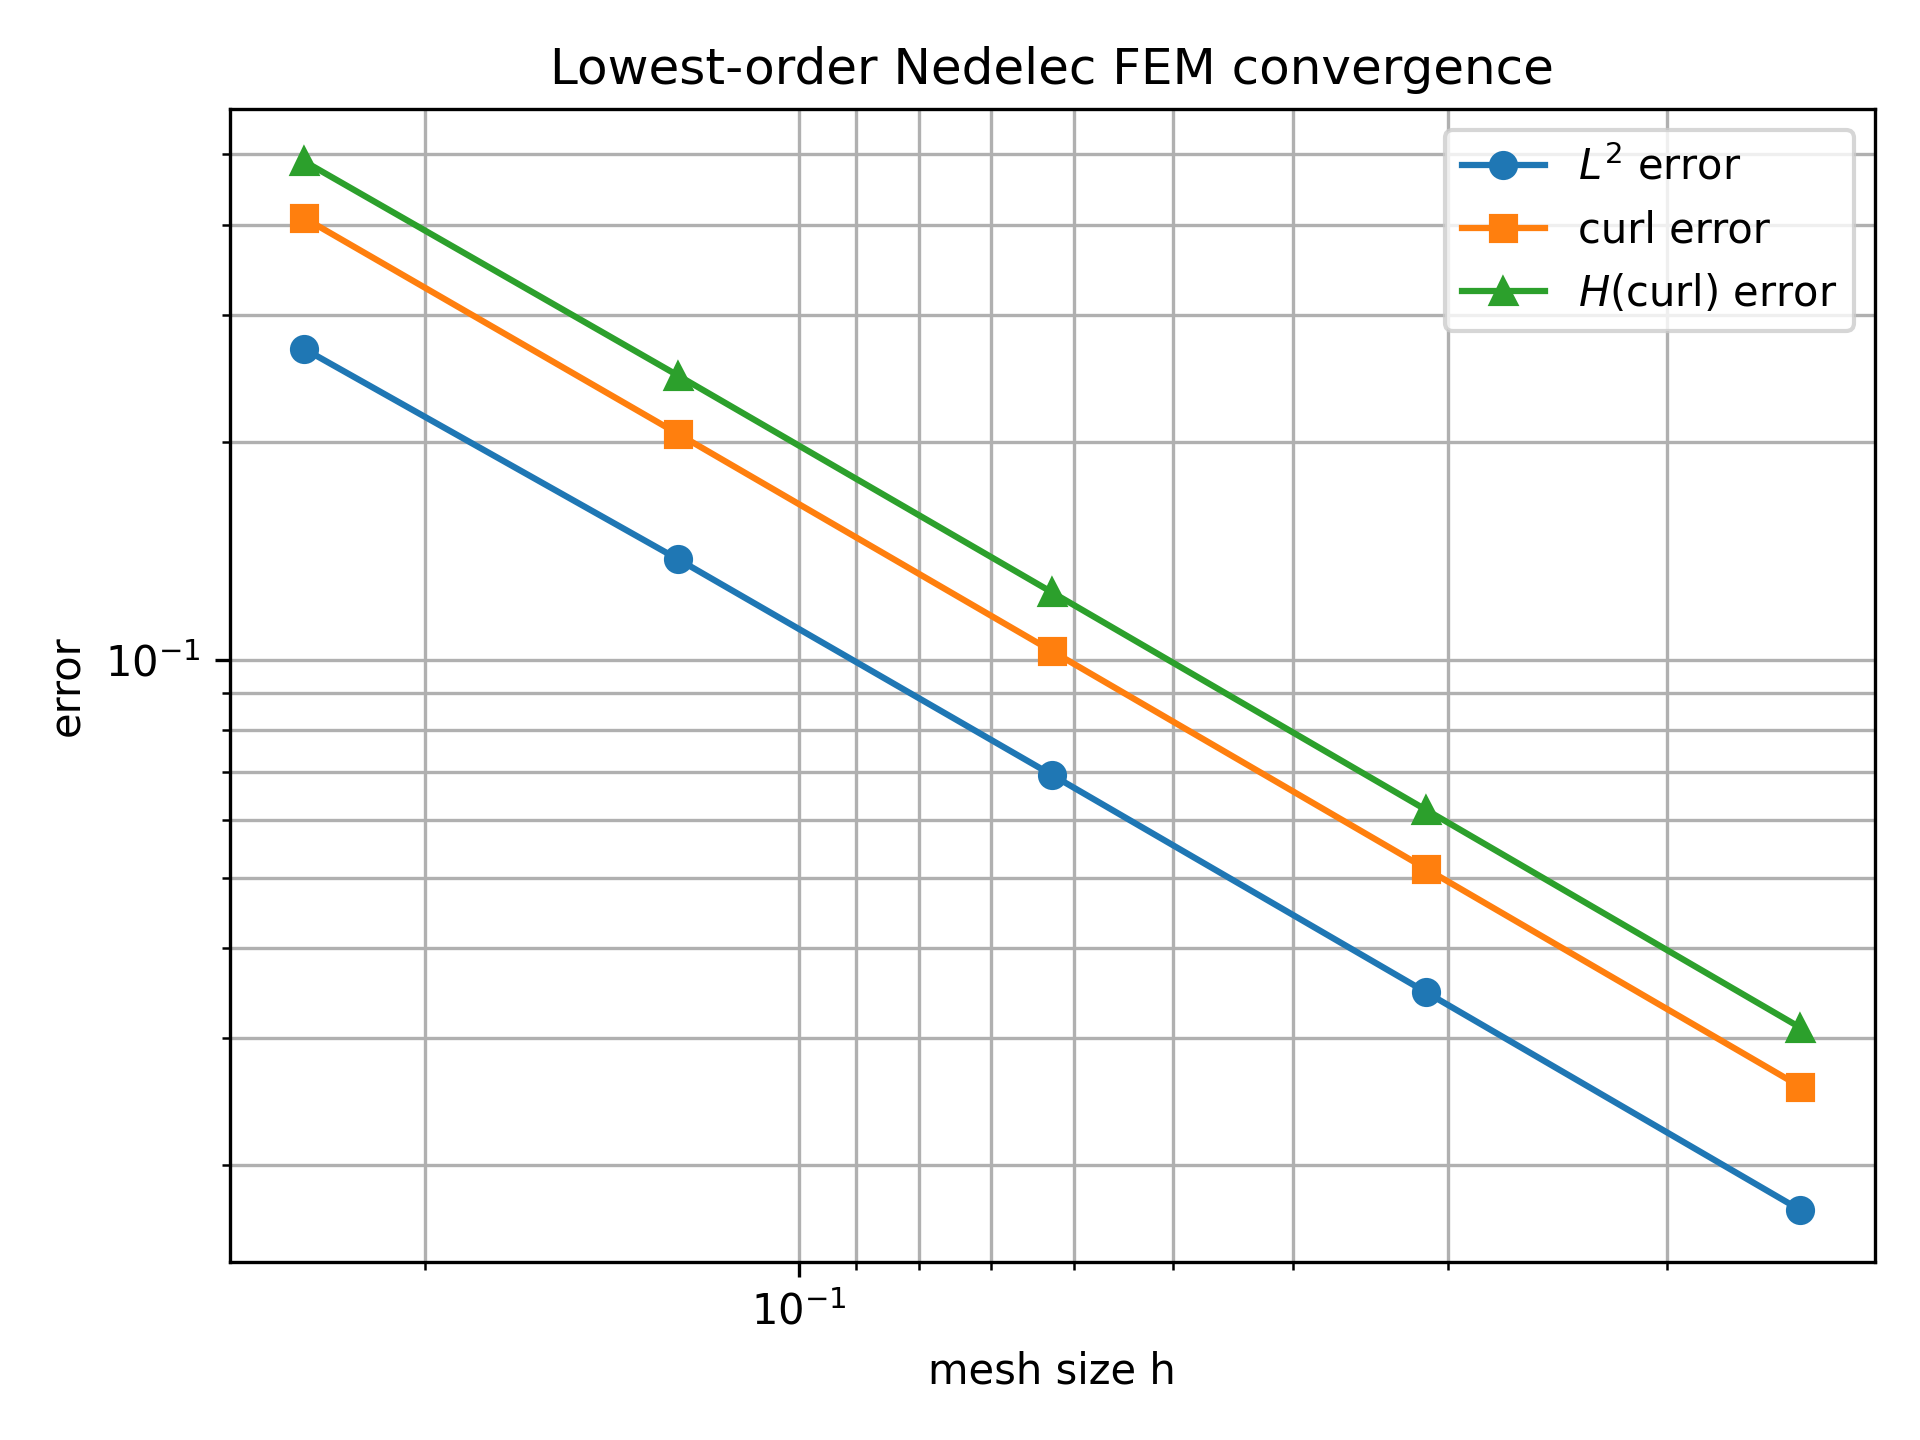
\includegraphics[width=0.78\textwidth]{figures/convergence.png}
\caption{最低阶 Nédélec 边缘元的误差收敛曲线}
\label{fig:nedelec_convergence}
\end{figure}

图 \ref{fig:nedelec_convergence} 给出了 $L^2$ 误差、旋度误差以及 $H(\curl)$ 误差随网格尺寸 $h$ 变化的双对数曲线.从图中可以看到,随着网格逐步加密,三类误差均稳定下降,并且在双对数坐标下基本呈直线分布.这说明数值解确实随着网格细化收敛到精确解.由于本文使用的是最低阶 Nédélec 边缘元,理论上在 $H(\curl)$ 范数下通常期望得到接近一阶的收敛速度；图中的误差曲线与这一理论预期一致.

同时可以观察到,$H(\curl)$ 误差曲线与旋度误差曲线较为接近.这是因为在本算例中旋度误差相对 $L^2$ 误差更大,对 $H(\curl)$ 范数的贡献占主导.因此,$H(\curl)$ 误差主要反映了旋度项的逼近精度.这也符合 Maxwell 问题的特点:旋度算子是方程中的主导微分算子,数值格式必须优先保证旋度结构的正确离散.

\begin{figure}[htbp]
\centering
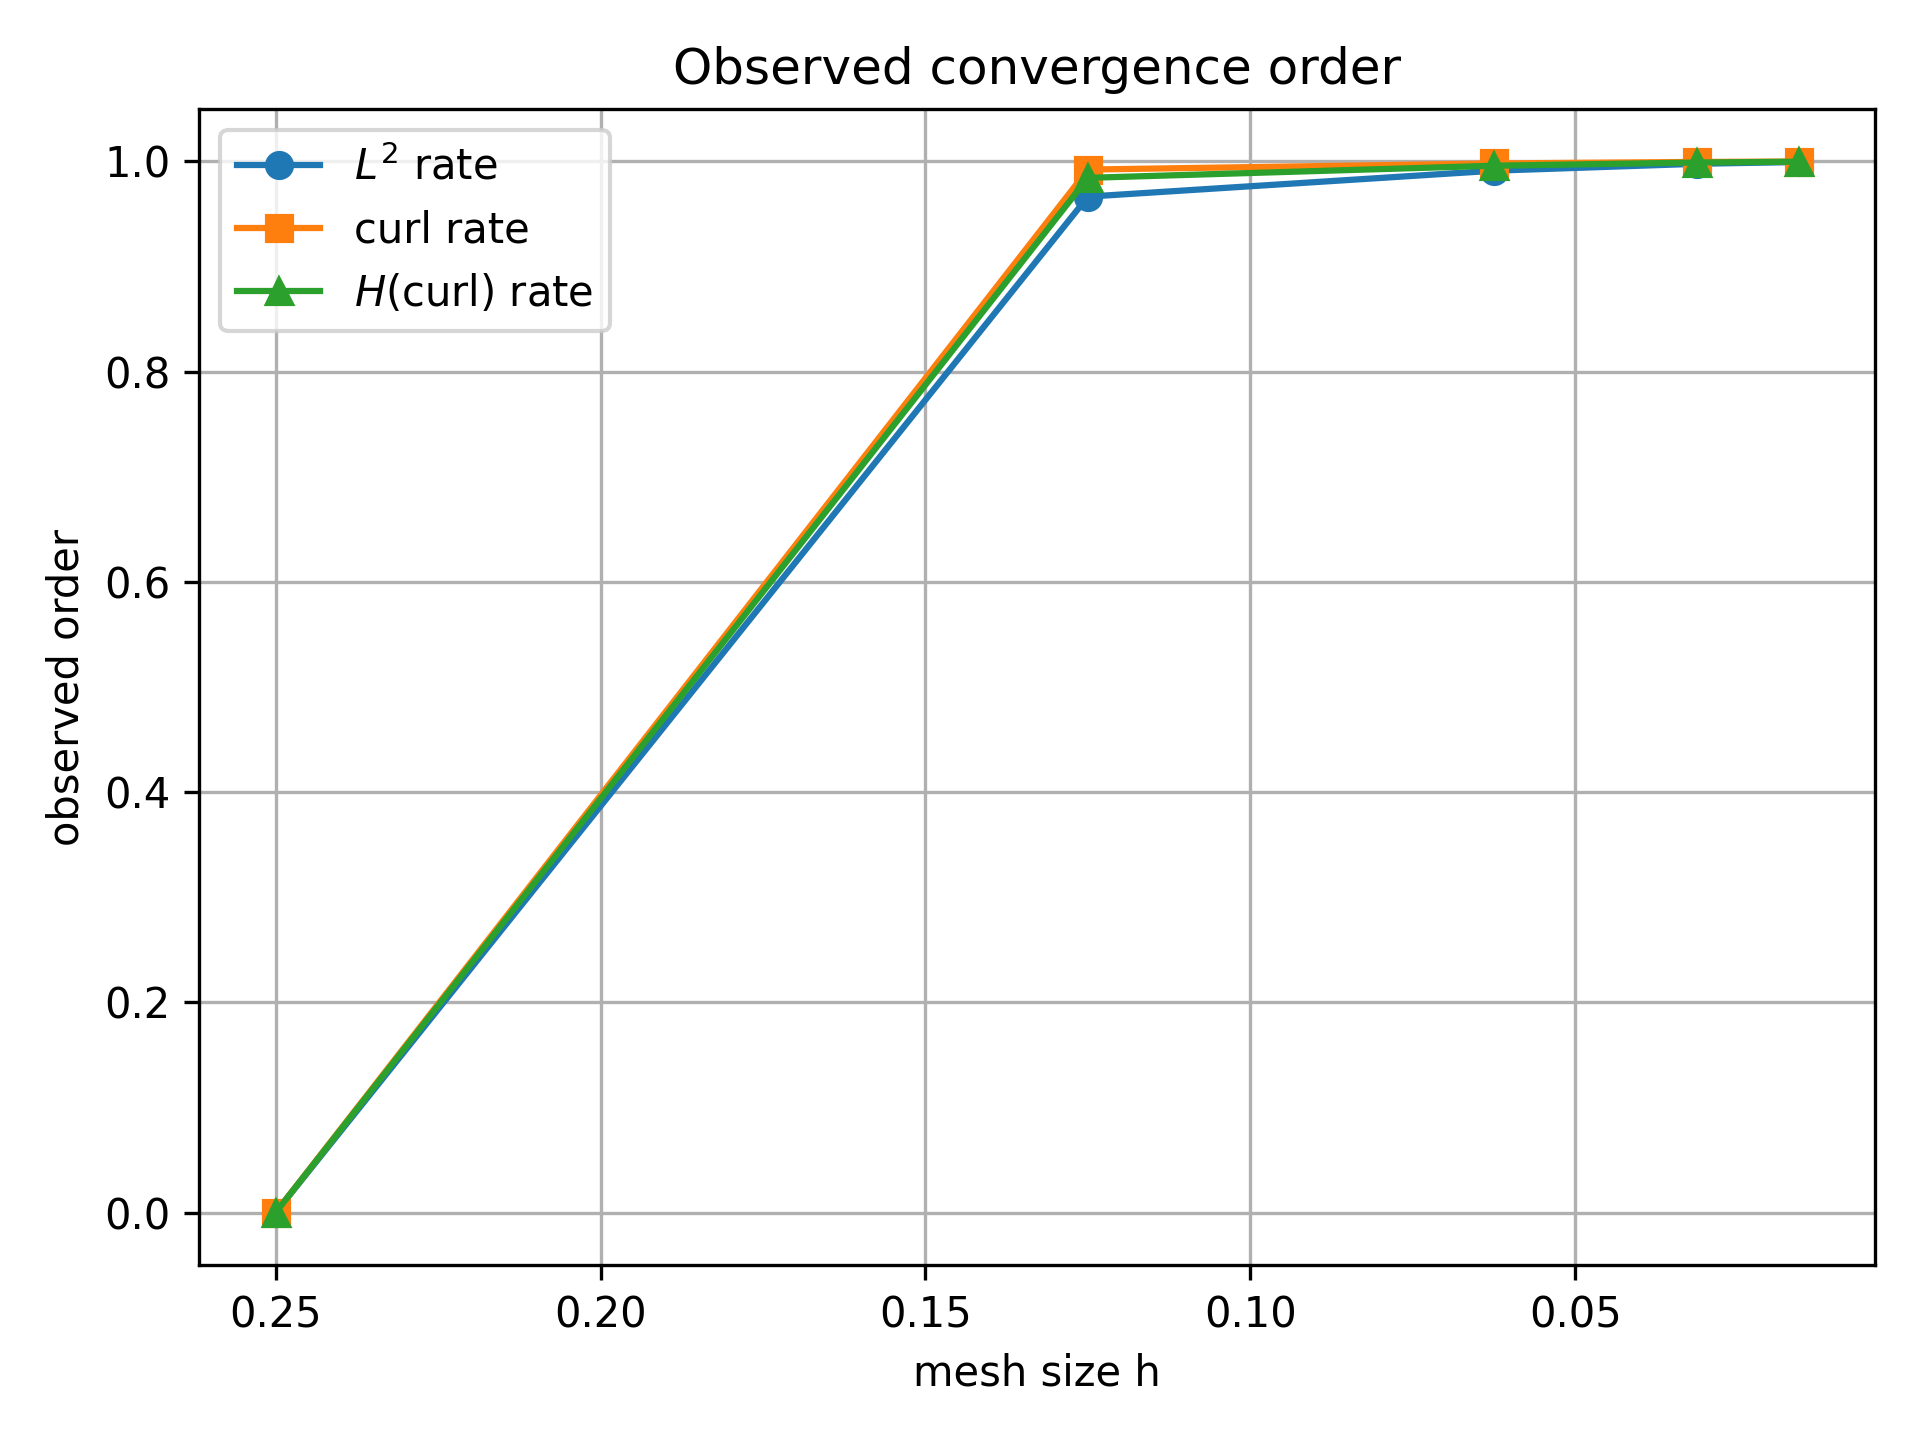
\includegraphics[width=0.78\textwidth]{figures/rates.png}
\caption{不同网格尺寸下的观测收敛阶}
\label{fig:nedelec_rates}
\end{figure}

图 \ref{fig:nedelec_rates} 给出了由相邻网格误差计算得到的观测收敛阶.第一层网格由于没有更粗网格作为比较对象,程序中将其收敛阶记为 $0$,该点不参与实际收敛性判断.从后续网格可以看到,$L^2$ 误差、旋度误差和 $H(\curl)$ 误差的观测收敛阶均逐渐接近 $1$.这说明在当前光滑制造解和规则三角网格条件下,最低阶 Nédélec 元表现出稳定的一阶收敛行为.

需要指出的是,这里的 $L^2$ 误差并未表现出明显高于一阶的超收敛现象.这是可以接受的,因为本文程序采用最低阶边缘元,并且电场自由度定义在边上而非节点上,数值场的重构方式与传统节点元不同.因此,更应关注 $H(\curl)$ 范数和旋度误差的收敛表现.从结果看,二者均接近一阶,说明离散格式与理论分析相吻合.

\begin{figure}[htbp]
\centering
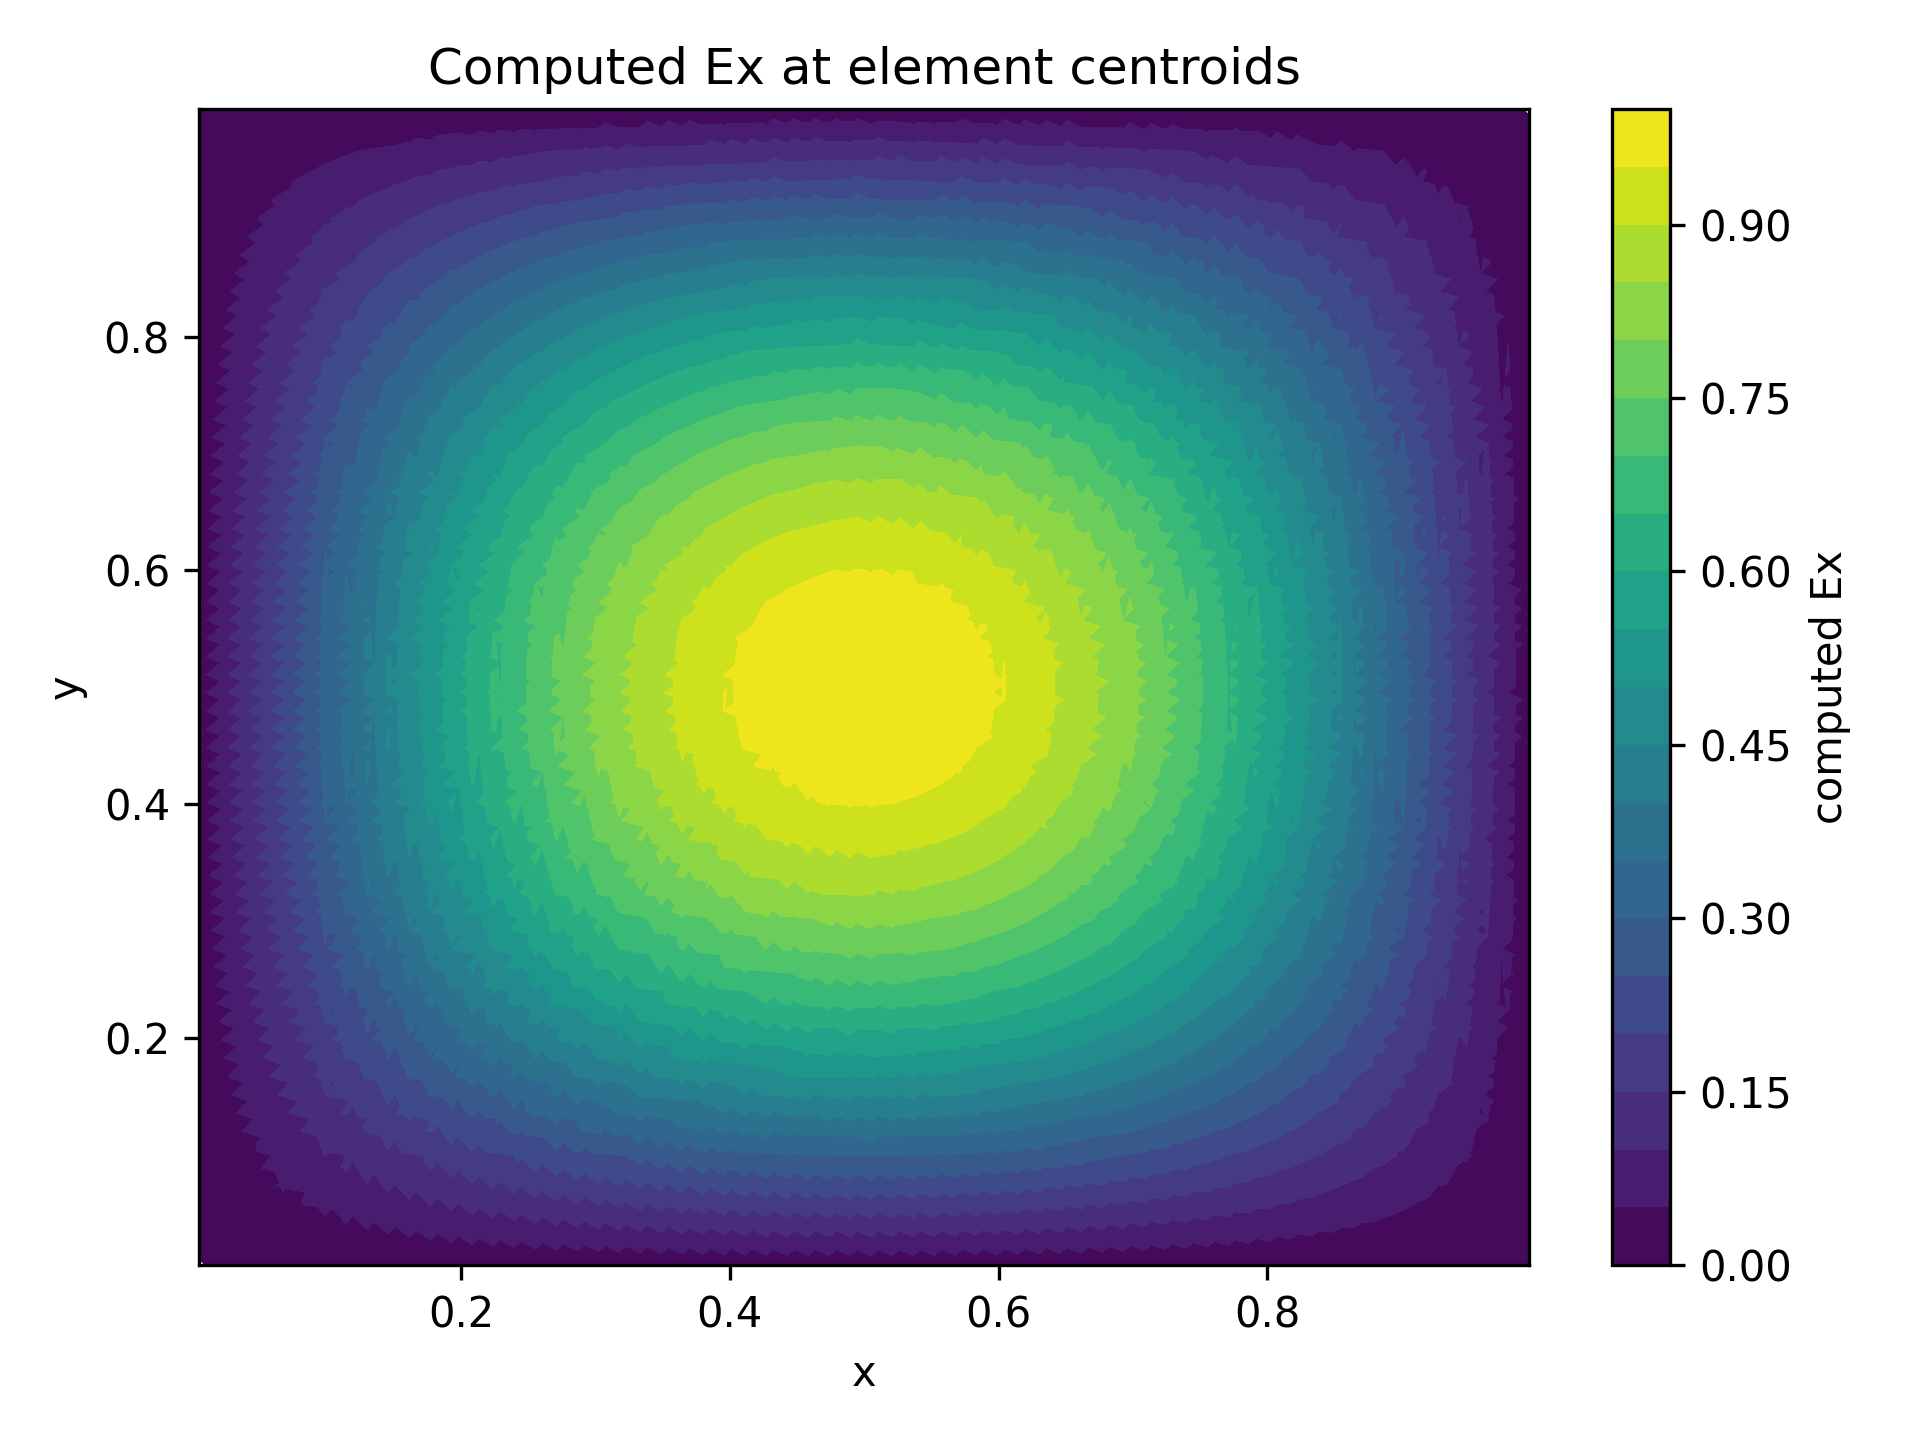
\includegraphics[width=0.76\textwidth]{figures/solution_Ex.png}
\caption{单元重心处计算得到的电场 $E_x$ 分量}
\label{fig:nedelec_ex}
\end{figure}

图 \ref{fig:nedelec_ex} 展示了最细网格上单元重心处计算得到的 $E_x$ 分量.由于制造解中
\[
E_x=\sin(\pi x)\sin(\pi y),
\]
其在边界处为零,在区域中心附近达到最大值.数值结果呈现出与精确解一致的空间分布:边界附近数值接近零,中心区域数值较大,并且整体关于区域中心具有对称性.这说明数值解不仅在误差范数意义下收敛,而且在场分布形态上也正确再现了精确解的主要特征.

\begin{figure}[htbp]
\centering
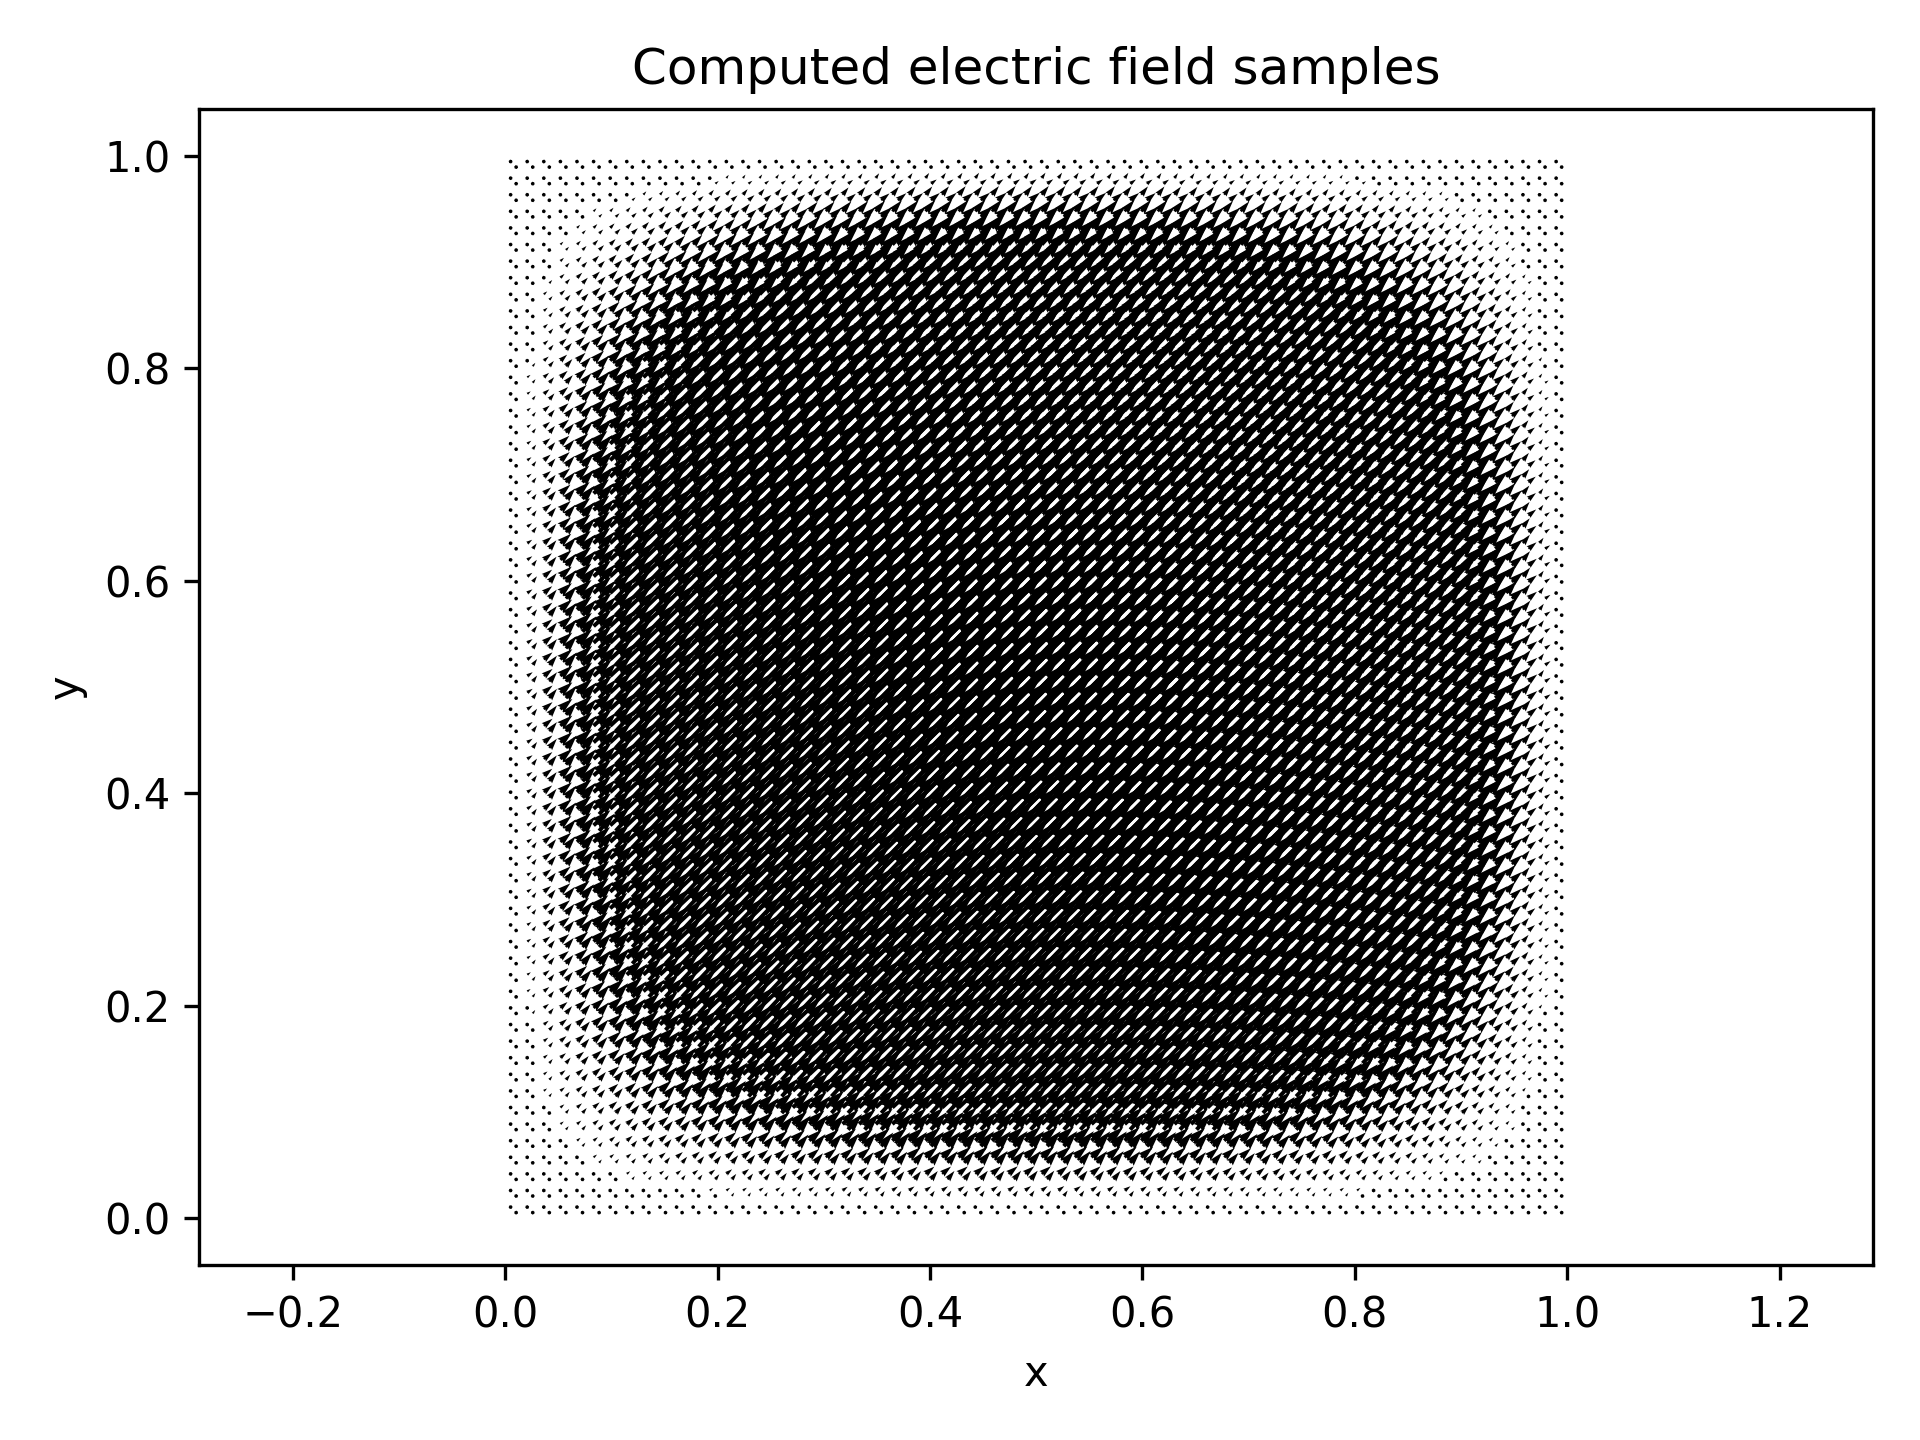
\includegraphics[width=0.78\textwidth]{figures/solution_quiver.png}
\caption{计算得到的二维电场矢量分布}
\label{fig:nedelec_quiver}
\end{figure}

图 \ref{fig:nedelec_quiver} 给出了二维电场的矢量分布.由于制造解满足 $E_x=E_y$,因此区域内部的电场方向主要沿 $(1,1)$ 方向分布.靠近边界时,$\sin(\pi x)\sin(\pi y)$ 逐渐趋近于零,因此箭头长度明显变小；在区域中心附近,电场幅值最大,箭头也最明显.这与图 \ref{fig:nedelec_ex} 中的标量云图相互印证.图中箭头数量较多是由于可视化时使用了较密的单元重心采样点,并不表示数值解存在振荡或不稳定.

综合上述数值结果可以看出,本文实现的二维最低阶 Nédélec 边缘元程序能够正确处理 PEC 边界条件,能够稳定逼近制造解,并在 $L^2$、旋度以及 $H(\curl)$ 范数下表现出接近一阶的收敛速度.这验证了前文弱形式推导、边缘元离散以及稀疏矩阵装配方法的正确性,也说明该实现可以作为进一步研究复杂二维电磁问题的基础.

\section{先验误差分析}

为了分析有限元近似解 $\E_h$ 与精确解 $\E$ 的误差,需要借助 Nédélec 边缘元的插值理论.设连续解满足
\[
\E\in V=H_0(\text{curl};\Omega),
\]
离散解满足
\[
\E_h\in V_h\subset V.
\]
设 $\Pi_h$ 为 Nédélec 插值算子.对于足够光滑的向量场 $\E$,插值函数 $\Pi_h\E$ 满足边自由度保持性质:
\[
\int_e
(\Pi_h\E)\cdot\tvec_e\,ds
=
\int_e
\E\cdot\tvec_e\,ds,
\qquad
\forall e\in\mathcal{E}_h,
\]
其中 $\mathcal{E}_h$ 表示网格边集合.该性质说明,Nédélec 插值匹配的是边上的切向积分,而不是节点函数值.

在适当正则性假设下,最低阶 Nédélec 插值具有如下估计:
\[
\|\E-\Pi_h\E\|_{[L^2(\Omega)]^2}
+
h\|\curl(\E-\Pi_h\E)\|_{L^2(\Omega)}
\le
C h^r
\left(
\|\E\|_{[H^r(\Omega)]^2}
+
\|\curl\E\|_{H^r(\Omega)}
\right),
\]
其中 $C$ 与网格尺寸 $h$ 无关,$r>0$ 取决于区域几何、材料系数和解的正则性.对于光滑区域和光滑系数,最低阶边缘元通常可以观察到接近一阶的收敛；而在凹角、尖角或材料跳跃界面附近,解可能出现奇异性,此时实际收敛阶往往低于一阶.

由 Galerkin 正交性可得
\[
a(\E-\E_h,\bm{v}_h)=0,
\qquad
\forall \bm{v}_h\in V_h.
\]
若问题在所考虑频率下满足稳定性条件,则由 Céa 型估计可得
\[
\|\E-\E_h\|_{H(\text{curl};\Omega)}
\le
C
\inf_{\bm{v}_h\in V_h}
\|\E-\bm{v}_h\|_{H(\text{curl};\Omega)}.
\]
取 $\bm{v}_h=\Pi_h\E$,可进一步得到
\[
\|\E-\E_h\|_{H(\text{curl};\Omega)}
\le
C h^r
\left(
\|\E\|_{[H^r(\Omega)]^2}
+
\|\curl\E\|_{H^r(\Omega)}
\right).
\]

该估计说明,误差不仅依赖于网格尺寸 $h$,还依赖于精确解的光滑性.在实际电磁计算中,场量常在几何奇点、材料界面或边界角点附近变化剧烈.若采用均匀网格细化,为了降低局部奇异区域的误差,往往需要在整个区域上增加大量自由度,计算成本较高.因此,后验误差估计驱动的自适应网格细化具有重要意义.

自适应网格细化的基本流程可概括为
\[
\text{求解}
\longrightarrow
\text{误差估计}
\longrightarrow
\text{标记单元}
\longrightarrow
\text{局部加密}
\longrightarrow
\text{重新求解}.
\]
对于 Maxwell 问题,误差指示子通常与单元残差、边界残差以及相邻单元之间的跳跃项有关.通过局部加密,可以在自由度增长较小的情况下提高整体计算精度.

\section{结论}

本文围绕二维频域 Maxwell 方程的有限元离散展开讨论,从数学模型、函数空间、弱形式、边缘元离散、稀疏矩阵实现以及误差估计等方面说明了 Nédélec 边缘元的必要性和优势.通过将问题限制在二维有界区域 $\Omega\subset\R^2$ 上,本文降低了模型复杂度,同时保留了 Maxwell 方程中最核心的旋度结构和切向连续性要求.

在理论方面,本文首先建立了带 PEC 边界条件的二维双旋强形式模型,并给出了二维旋度算子的定义.随后引入 $H(\text{curl};\Omega)$ 与 $H_0(\text{curl};\Omega)$ 空间,通过二维旋度 Green 公式推导了弱形式.该弱形式降低了对电场经典可微性的要求,使问题能够在更自然的能量空间中进行分析.

在离散方面,本文采用三角剖分上的最低阶第一类 Nédélec 边缘元.该方法以边上的切向积分作为自由度,能够保持跨单元边界的切向连续性,并避免传统节点元在 Maxwell 问题中可能产生的非物理伪模态.离散后得到的矩阵系统具有高度稀疏性,可通过三元组批量装配和稀疏求解器高效求解.

最后,本文结合制造解算例展示了误差收敛曲线、电场分量云图和矢量场分布.数值结果表明,在光滑解和规则三角网格条件下,最低阶 Nédélec 边缘元在 $L^2$、旋度以及 $H(\curl)$ 范数下均表现出接近一阶的收敛速度.进一步地,本文给出了基于 Nédélec 插值和 Céa 型估计的先验误差分析,说明数值解的收敛速度不仅取决于网格尺寸,也受到区域几何奇点和材料不连续性的影响.在更复杂的计算电磁问题中,结合后验误差估计的自适应网格细化将是进一步提高精度和效率的重要方向.

总体而言,二维 Maxwell 模型虽然是对完整三维电磁问题的简化,但它完整保留了 $H(\text{curl})$ 空间、PEC 边界条件、Nédélec 边自由度和稀疏矩阵求解等关键结构.通过该模型,可以较系统地理解边缘元方法在计算电磁学中的数学基础与实现路径.

\end{document}
